% https://github.com/raulmur/ORB_SLAM2
% https://ieeexplore.ieee.org/document/7946260
ORB\hyp{}SLAM2 is a real\hyp{}time \acs{slam} algorithm suitable for monocular, stereo and \acs{rgbd} cameras. It can handle loop closures and has relocalization capabilities. ORB-SLAM2 was developed in 2017 by Ra\'ul Mur\hyp{}Artal, Juan D. Tard\'os, J. M. M. Montiel, and Dorian G\'alvez\hyp{}L\'opez. The algorithm returns a sparse \acs{3d} reconstruction with true scale. \cite{orb_slam2_github} \cite{mur_orb_slam_2}

The algorithm has an option to compiled with \acs{ros}. Therefore it seemed a reasonable option for this project. After the implementation and some experimenting with ORB\hyp{}SLAM2, it became clear that the density of the point cloud was to sparse for this project.

\begin{figure}[!h]
  \centering
  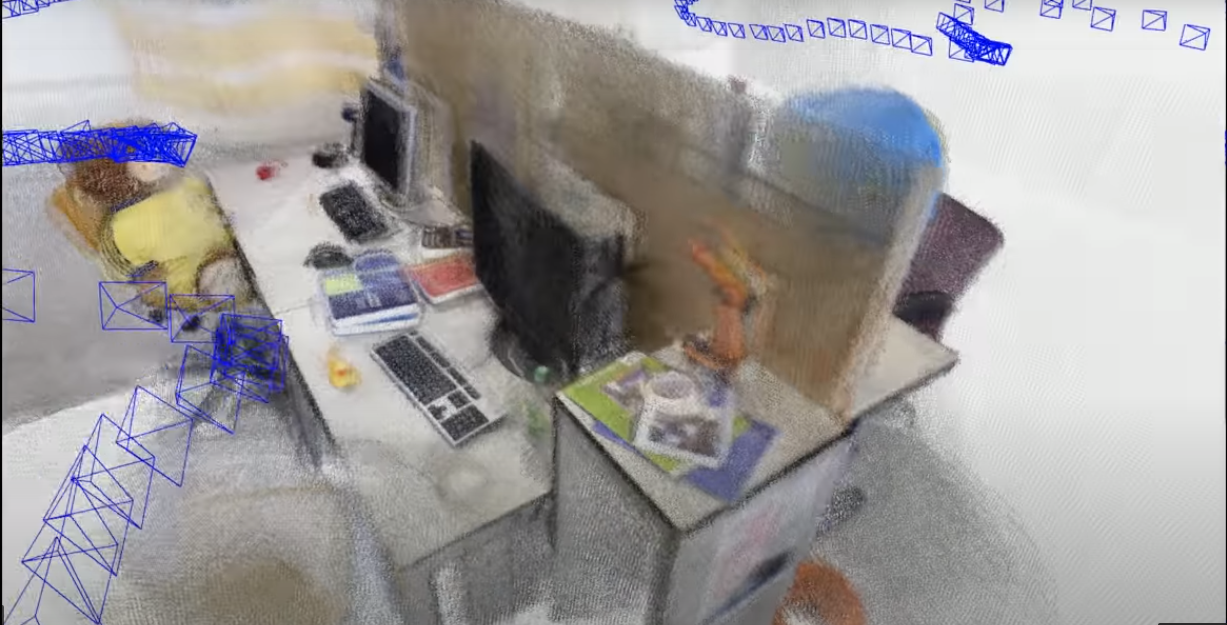
\includegraphics[width=\linewidth]{images/orb_slam2.png}
  \caption{ORB\hyp{}SLAM2 example \cite{orb_slam2_youtube}}
\end{figure}